\documentclass[11pt,a4paper]{scrartcl}
\usepackage[czech]{babel}
\usepackage[utf8]{inputenc}
\usepackage{graphicx}
\usepackage{epstopdf}
\usepackage{float}
\graphicspath{{./img/}}

\begin{document}
	\title{Semestrální práce z předmětu KIV/NET}
	\subtitle{Dungeon hra}
	\author{Zdeněk Valeš}
	\date{7.4.2018}
	\maketitle
	\newpage
	
	\section{Zadání}
	V jazyce C\# vytvořte jednoduchou hru, ve které bude hráč procházet bludištěm (dungeonem). Cílem hráče je najít východ dříve než protihráči (počítač). Uživatelské rozhraní bude realizováno technologií WPF. Aplikace bude obsahovat jednoduchý editor map s možností importovat (exportovat) mapy do (ze) souboru.
	
	\subsection{Cíl projektu}
	Cílem projektu je vytvoření jednoduché hry. Při tvorbě aplikace se seznámím se základními technologiemi a postupy, které se v této oblasti používají.
	
	\subsection{Požadavky}
	Aplikace má následující funkční požadavky:
	\begin{itemize}
		\item Vytvořit novou hru o zadané velikosti mapy (šířka, výška), se zadaným počtem soupeřů (ovládaných počítačem).
		
		\item Hráč může při procházení mapou sbírat předměty, které mu pomáhají ve hře (zbroj, zbraně, klíče, ...).
		
		\item Vyhrát hru nalezením cílového pole, případně hru prohrát, pokud toto pole nalezne soupeř.
		
		\item Vytvořit mapu v editoru a vyexportovat ji do souboru.
		
		\item Importovat mapu ze souboru.
		
		\item Možnost hru uložit a později opět nahrát.
	\end{itemize}
	
	\section{Analýza}
	
	Jádro aplikace se skládá ze 3 hlavních komponent. 1. komponenta obsahuje vše potřebné pro práci s herní mapou, 2. obsahuje herní objekty (včetně hráčů), 3. pak samotnou instanci hry.
	
	\subsection{Komponenta pro práci s herní mapou}
	Herní mapa je tvořena maticí herních polí. Každé herní pole má čtyři východy (podle světových stran), které mohou být v otevřeném, zavřeném, nebo neexistujícím stavu. Jednotlivé stavy jsou popsány v následujícím výčtu:
	
	\begin{itemize}
		\item \textit{OTEVŘENÝ}: východ je otevřený a blok je možné tímto východem opustit, nebo do něj přijít.
		
		\item \textit{ZAVŘENÝ}: východ je zavřený a k jeho otevření je potřeba získat klíč (a mít jej v inventáři). Pokud je východ jednou otevřen pomocí klíče, nemůže být už znovu zavřen a každý jím může projít.
		
		\item \textit{NEEXISTUJÍCÍ}: východ v tomto směru neexistuje. V uživatelském rozhraní bude reprezentován například zdí.
	\end{itemize}
	
	\paragraph{Generování mapy}
	V aplikace je dungeon vnímán jako podzemní bludiště (například systém jeskyní) a k vytvoření herní mapy je k dispozici generátor. 
	
	Ke generování mapy je použit algoritmus postupného probourávání, kdy na začátku je matice herních polí se všemi východy ve stavu \textit{NEEXISTUJÍCÍ} a algoritmus postupně prochází celou mapu a náhodně probourává stěny jednotlivých bloků. Výsledkem je bludiště bez izolovaných míst -- platí tedy, že mezi každými dvěma bloky existuje cesta. To mimo jiné zjednodušuje pozdější náhodou volbu startovacích pozic hráčů, monster a umístění předmětů, protože nemůže nastat situace kdy by například hráč nemohl dojít do cíle.
	
	\subsection{Komponenta pro práci s herními objekty}
	Všechny objekty, které mohou být umístěny na mapu, a v případě hráčů a monster se po ní i pohybovat, jsou v rámci aplikace souhrnně nazvané jako 'herní objekty'. Jsou rozděleny do dvou podmnožin: živé a neživé objekty, kde živé objekty představují hráče (člověka i počítač), neživé pak předměty které lze na mapě sebrat (například zbraň).
	
	Všechny předměty mají dvě společné vlastnosti: hrací blok, na kterém jsou umístění a název. Základní struktura herních objektů je naznačena na obrázku \ref{fig:game-obj}. 
	
	\begin{figure}[H]
		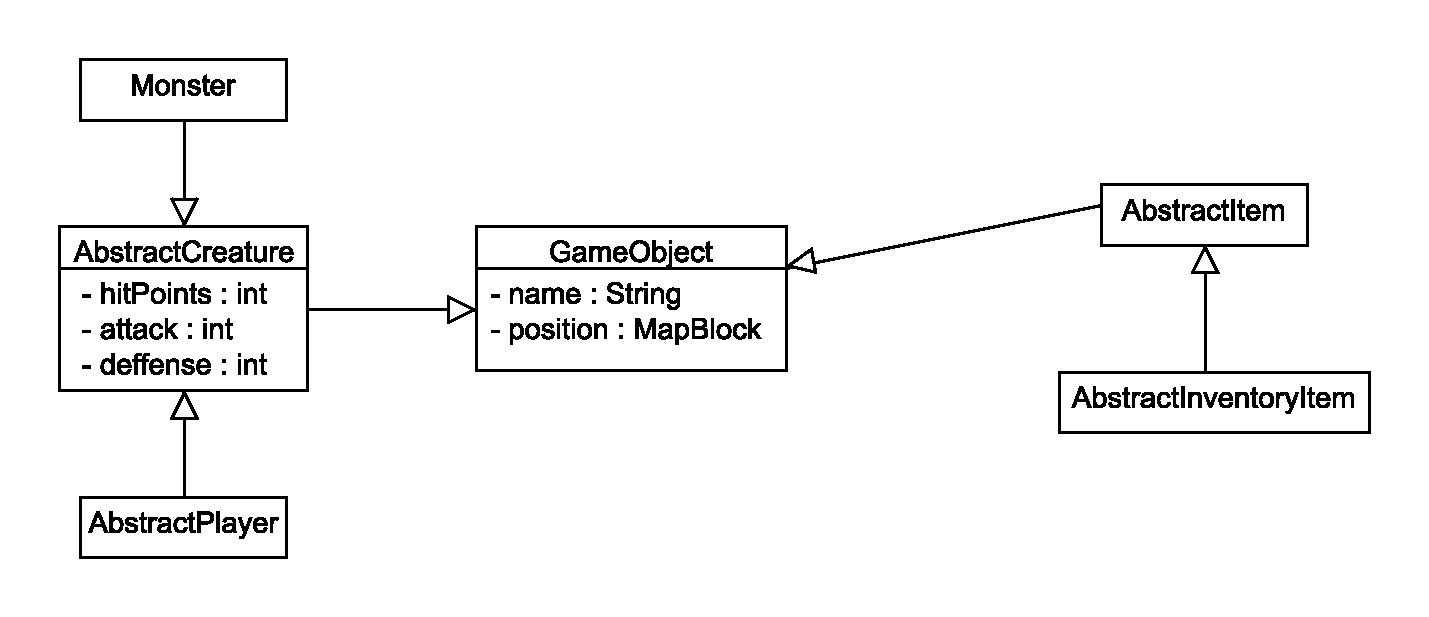
\includegraphics[width=140mm]{core-game-objects-simple}
		\caption{Struktura herních objektů}
		\label{fig:game-obj}
	\end{figure}
	
	\subsubsection{Předměty}
	Předměty může mít hráč buďto nasazené (na obrázku \ref{fig:game-obj} \textit{AbstractItem}), nebo je může nosit v inventáři (na obrázku \ref{fig:game-obj} \textit{AbstractInventoryItem}). 
	
	V případě nositelných předmětů se jedná o zbraně a brnění. Ty dávají hráči bonusy k jeho základním schopnostem (zdraví, život, útok) a hráč může mít v jeden okamžik nasazenou pouze jednu zbroj (respektive zbraň).
	
	Oproti tomu v inventáři může hráč nosit libovolný počet stejných věcí (počet je omezen kapacitou inventáře). Speciální věc v inventáři je pak klíč, který slouží k odemčení zavřených průchodů mezi herními bloky.
	
	\subsubsection{Monstra a hráči}
	
	
	\subsection{Komponenta pro práci s instancí hry}
	
	něco o akcích, akce házejí výjimky - reakce na ně v UI
	
	\section{Implementace}
	
	 
	\section{Závěr}
	
\end{document}
